\documentclass[letterpaper,11pt]{report}
% Change margins to 1 inch on all sides
\addtolength{\oddsidemargin}{-.875in}
\addtolength{\evensidemargin}{-.875in}
\addtolength{\textwidth}{1.75in}
\addtolength{\topmargin}{-.875in}
\addtolength{\textheight}{1.75in}
\usepackage{float}
\usepackage{graphicx}
\usepackage{footnote}
\usepackage{longtable}
\usepackage{multirow}
\usepackage{tablefootnote}
\usepackage{tabularx}
\usepackage{url}
\DeclareGraphicsExtensions{.pdf,.png,.jpg}

%%%%%%%%%%Start of report
\begin{document} 
\begin{savenotes}
\pagestyle{plain}
\title{CS896 Introduction to Web Science\\Fall 2013\\Report for Assignment 4}
\author{Corren G. McCoy}
 
\date{October 10, 2013}
\maketitle

\renewcommand*\thesection{\arabic{section}}
\setcounter{section}{0}

\setcounter{tocdepth}{4}
\tableofcontents
 \listoffigures
% \listoftables
\newpage


%%%%%%%%%%Chapter Exercises
\section{Question 1}
\subsection{Problem}From your list of 1000 links, choose 100 and extract all of the links from those 100 pages to other pages. For each URI, create a text file of all of the outbound links from that page to other URIs.
\subsection{Response}We used Python to traverse our list of 1000 URIs and Beautiful Soup to retrieve the HTML source code for the URI. We then searched the source for the URI and title for any outbound links. If anchor tags with the href attribute were found, the referring site and list of outbound links were written to a text file as shown in Appendix \ref{chap:file1}.  For each referring URI, internal page links (i.e., navigation) were ignored along with duplicate references to the same external URI. We also excluded anchor tags that referenced JavaScript. The Python source code for \emph{extractHREF} is shown in Appendix \ref{chap:extractHREF}. The 100 sites of interest were chosen based on a manual review of the original list of 1000 links. To compile our list of 100, we grouped the URIs into the following categories:
\begin{itemize}
\item blogs from a common domain (e.g., www.wordpress.com, www.blogspot.com);
\item political sites (e.g., www.usa.gov, www.breitbart.com);
\item print or television media (e.g., www.latimes.com, www.nytimes.com);
\item sites with a large web presence (e.g., www.yahoo.com, www.gatesfoundation.org); and
\item other miscellaneous entities (e.g., www.myitworks.com).
\end{itemize}

%%%%%%%%%%Chapter Exercises
\section{Question 2}
\subsection{Problem}Using these 100 files, create a single GraphViz `dot' file of the resulting graph.
\subsection{Response}The \emph{extractHREF} code was also used to create the `dot' file. Each URI, outbound link, and title attribute were combined to generate the node pairs and label required for the graph. After processing the 100 files, approximately 7200 node pairs were extracted. A portion of the GraphViz file output is shown below.

\begin{verbatim}
digraph twitter { 
size="6,6"; 
node [color=lightblue2, style=filled];
"http://www.usa.gov/"->"http://business.usa.gov" 
[label="Business"];
"http://www.usa.gov/"->"http://publications.usa.gov/" 
[label="Consumer Publications"];
"http://www.usa.gov/"->"http://travel.state.gov/passport/passport_1738.html" 
[label="Apply for a Passport"];
\end{verbatim}

%%%%%%%%%%Chapter Exercises
\section{Question 3}
\subsection{Problem}Load the `dot' file and use Gephi to:
\begin{itemize}
	\item visualize the list
	\item calculate HITS and PageRank
	\item avg degree
	\item network diameter
	\item connected components
\end{itemize}
Put the resulting graphs in your report.
\subsection{Response}As suggested in the assignment description, we reviewed our list of 1000 URIs and attempted to choose 100 which might display a high-level of connectivity. We then created a project in Gephi to visualize the network mapping. After importing the `dot' file, we performed the following steps using the insight obtained from an online Gephi tutorial\footnote{\url{http://pegasusdata.com/2013/01/10/facebook-friends-network-mapping-a-gephi-tutorial/}}.
\begin{itemize}
\item First, we eliminated any noise in the model by applying a filter to reduce the network to its largest, connected component. This step eliminated about 100 node pairs from the graph. These nodes could not be reached from any other nodes.
\item Second, we experimented with the node size by varying the size based on the degree.
\item Third, for the initial layout, we started with the Fruchterman Reingold algorithm, which uses attraction-repulsion to separate the nodes. Applying this algorithm allowed us to see the initial formation of any communities.
\item Fourth, we used the ForceAtlas 2 algorithm to further disperse the groups and add space around the larger nodes.
\item Fifth, since our `dot' file does not actually contain any categories as part of the data, we used node color to distinguish nodes based on the degree.
\item Finally, to further detect any communities, we used the Gephi statistics to calculate modularity classes (i.e., subnetworks). Node colors were then applied based on the density of the class. Because our network contains thousands of nodes, the option to display edge labels was turned off to maintain the readability of the graph. 
\end{itemize}
\paragraph{}As shown in Figure \ref{fig:ModularityClassGraph}, we observed one very dominant community which contains a cluster of over 21 percent of the network's nodes. This community represents the outgoing links from the Yahoo! web portal \url{http://www.yahoo.com}. No other community is comparable in size with most of the smaller subnetworks consisting of 4 percent or less. To assist with identification, Figure \ref{fig:ModularityLegend} shows a portion of the legend for the top 10 communities. We used the Gephi statistical functions to produce the remaining graphs. However, because we started with only 100 URIs, the additional graphs are sparse and do not convey a signicant amount of information about our network.

\begin{itemize}
	\item visualize the list, Figure \ref{fig:ModularityClassGraph};
	\item calculate HITS and PageRank, Figures \ref{fig:pageranks}, \ref{fig:authorities} and \ref{fig:hubs};
	\item avg degree, Figures \ref{fig:DegreeDistribution}, \ref{fig:IndegreeDistribution} and \ref{fig:OutDegreeDistribution};
	\item network diameter, Figures \ref{fig:Betweenness Centrality Distribution}, \ref{fig:Closeness Centrality Distribution}, and \ref{fig:Eccentricity Distribution}; and
	\item connected components, Figure \ref{fig:cc-size-distribution}.
\end{itemize}

\begin{figure}[htbp]
	\centering
		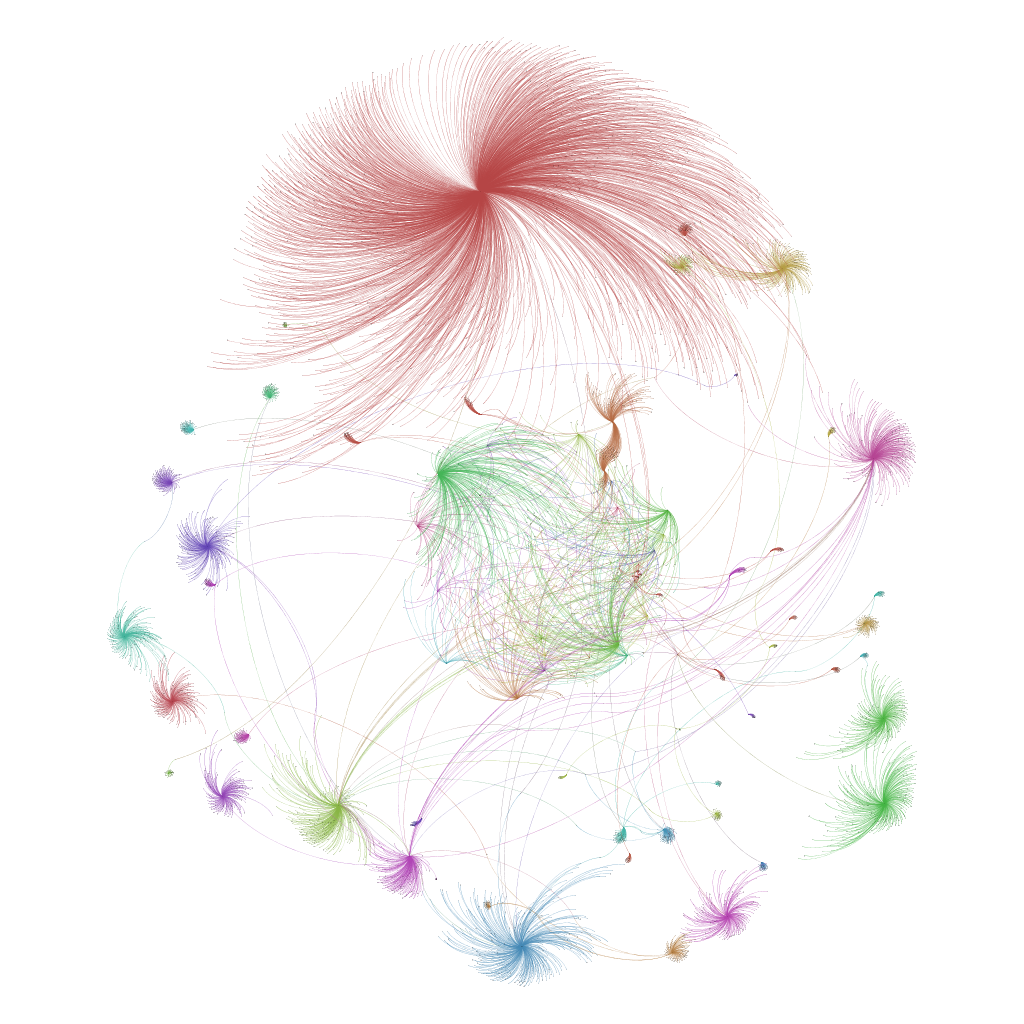
\includegraphics[width=0.60\textwidth]{ModularityClassGraph.png}
	\caption{Twitter Network Grouped by Modularity Class}
	\label{fig:ModularityClassGraph}
\end{figure}

\begin{figure}[htbp]
	\centering
		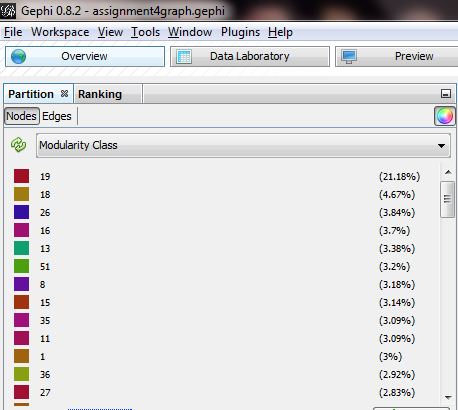
\includegraphics{ModularityLegend.png}
	\caption{Modularity Legend}
	\label{fig:ModularityLegend}
\end{figure}

\begin{figure}[htbp]
	\centering
		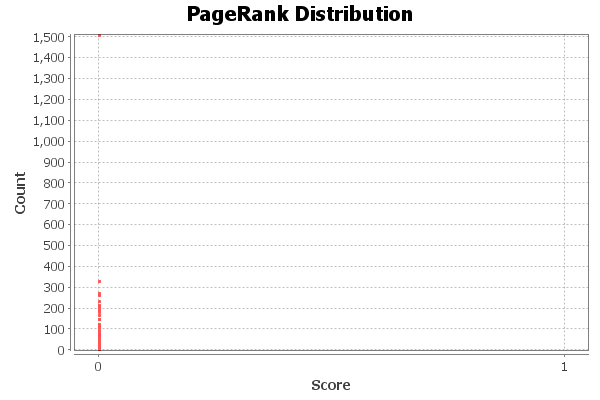
\includegraphics[width=0.60\textwidth]{pageranks.png}
	\caption{PageRank}
	\label{fig:pageranks}
\end{figure}

\begin{figure}[htbp]
	\centering
		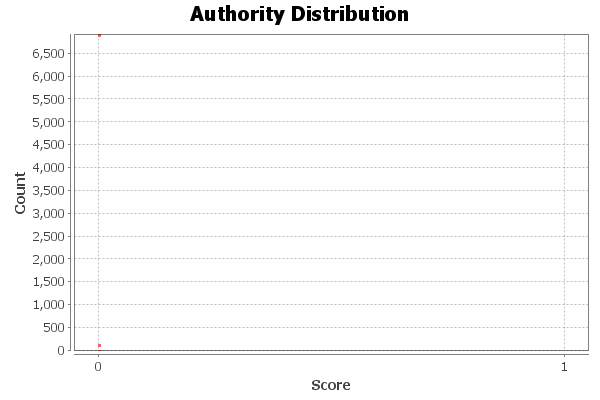
\includegraphics[width=0.60\textwidth]{authorities.png}
	\caption{HITS - Authority Distribution}
	\label{fig:authorities}
\end{figure}

\begin{figure}
	\centering
		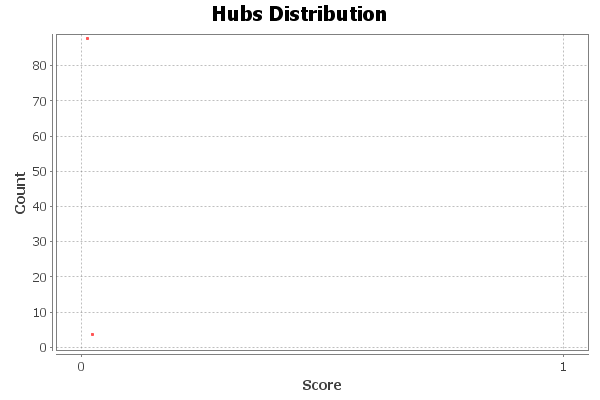
\includegraphics[width=0.60\textwidth]{hubs.png}
	\caption{HITS - Hubs Distribution}
	\label{fig:hubs}
\end{figure}

\begin{figure}[htbp]
	\centering
		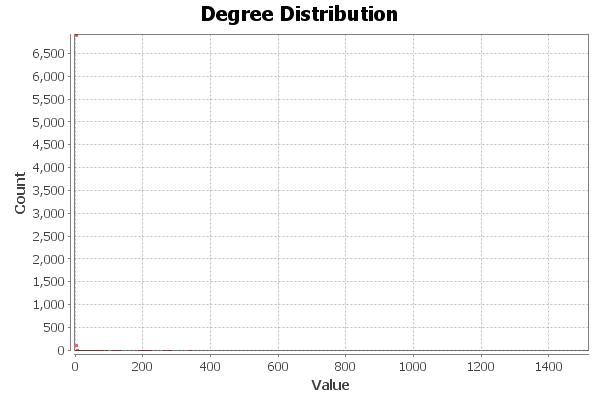
\includegraphics[width=0.60\textwidth]{DegreeDistribution.png}
	\caption{Avg Degree - Degree Distribution}
	\label{fig:DegreeDistribution}
\end{figure}


\begin{figure}[htbp]
	\centering
		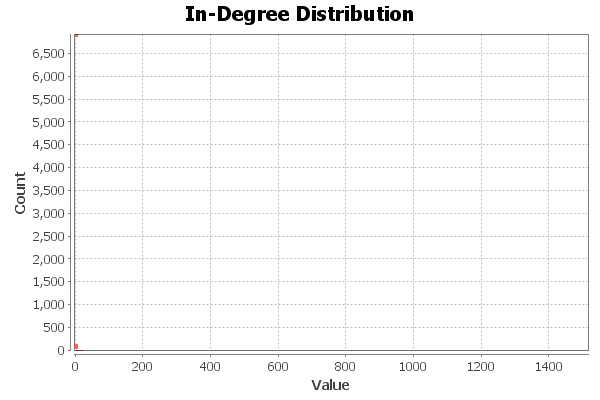
\includegraphics[width=0.60\textwidth]{IndegreeDistribution.png}
	\caption{Avg Degree - Indegree Distribution}
	\label{fig:IndegreeDistribution}
\end{figure}


\begin{figure}[htbp]
	\centering
		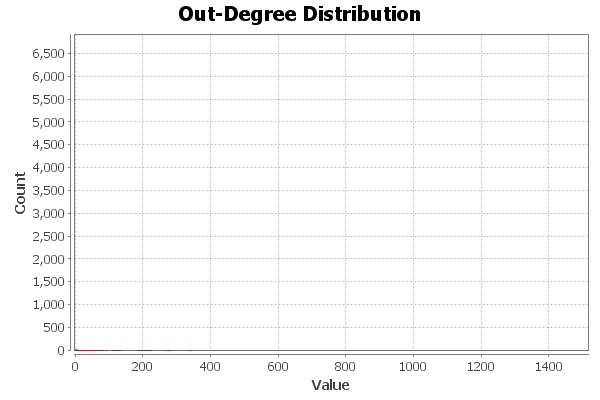
\includegraphics[width=0.60\textwidth]{OutDegreeDistribution.png}
	\caption{Avg Degree - Out Degree Distribution}
	\label{fig:OutDegreeDistribution}
\end{figure}


\begin{figure}
	\centering
		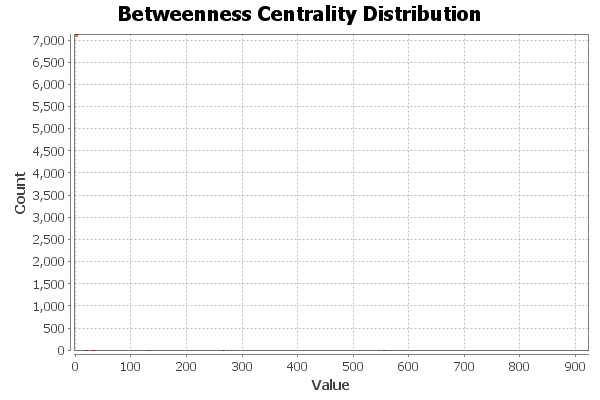
\includegraphics[width=0.60\textwidth]{BetweennessCentralityDistribution.png}
	\caption{Network Diameter - Betweenness}
	\label{fig:Betweenness Centrality Distribution}
\end{figure}

\begin{figure}[htbp]
	\centering
		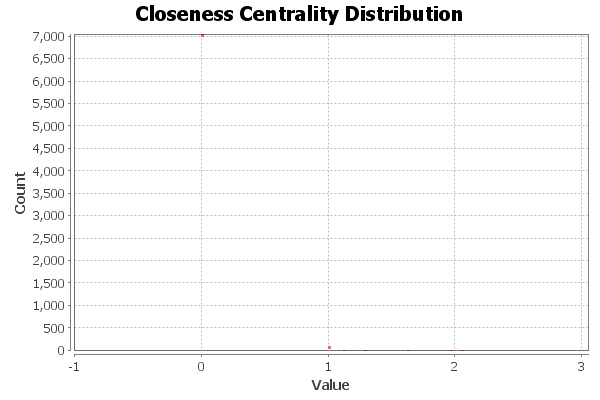
\includegraphics[width=0.60\textwidth]{ClosenessCentralityDistribution.png}
	\caption{Network Diameter - Closeness}
	\label{fig:Closeness Centrality Distribution}
\end{figure}

\begin{figure}[htbp]
	\centering
		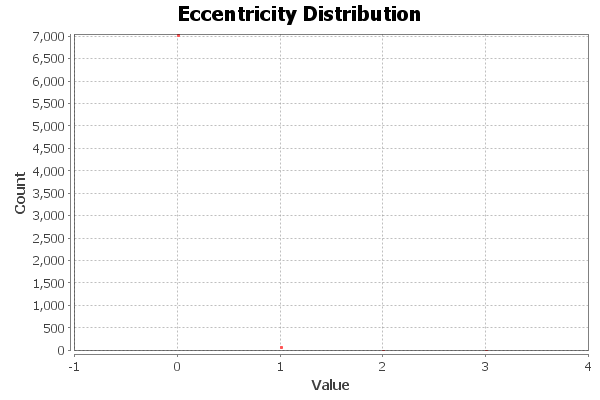
\includegraphics[width=0.60\textwidth]{EccentricityDistribution.png}
	\caption{Network Diameter - Eccentricity}
	\label{fig:Eccentricity Distribution}
\end{figure}



\begin{figure}[htbp]
	\centering
		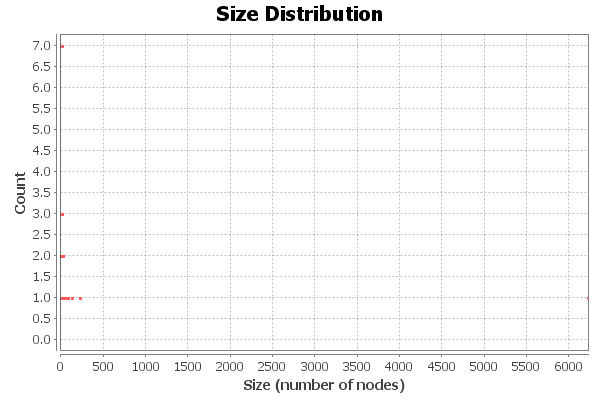
\includegraphics[width=0.60\textwidth]{cc-size-distribution.png}
	\caption{Connected Components}
	\label{fig:cc-size-distribution}
\end{figure}


\end{savenotes}

% produce the bibliography for the citations in your paper.
\bibliographystyle{abbrv}
\bibliography{cmccoy}

\appendix
\addcontentsline{toc}{chapter}{Appendices}

%%Appendix A
\chapter{Python Source - extractHREF.py} \label{chap:extractHREF}
\input{extractHREF.py}
\chapter{Sample URI file} \label{chap:file1}
\input{file1.txt}



\end{document} 
%%%%%%%%%%Ed of report
